\documentclass[a4 paper]{article}
\usepackage[a4paper, total={6in, 9.2in}]{geometry}
% Set target color model to RGB
% \usepackage[inner=2.0cm,outer=2.0cm,top=2.5cm,bottom=2.5cm]{geometry}
\usepackage{setspace}
\usepackage[rgb]{xcolor}
\usepackage{float}
\usepackage{verbatim}
\usepackage{subcaption}
\usepackage{amsgen,amsmath,amstext,amsbsy,amsopn,tikz,amssymb,tkz-linknodes}
\usepackage{fancyhdr}
\usepackage{hyperref}
\usepackage{amsmath}
\usepackage{hyperref}
% \usepackage{rotating}

%\usetikzlibrary{through,backgrounds}
\hypersetup{%
pdfauthor={Sawan Singh Mahara},%
pdftitle={Homework},%
pdfkeywords={Tikz,latex,bootstrap,uncertaintes},%
pdfcreator={PDFLaTeX},%
pdfproducer={PDFLaTeX},%
}
%\usetikzlibrary{shadows}
% \usepackage[francais]{babel}
\usepackage{booktabs}
\newcommand{\ra}[1]{\renewcommand{\arraystretch}{#1}}

\newtheorem{thm}{Theorem}[section]
\newtheorem{prop}[thm]{Proposition}
\newtheorem{lem}[thm]{Lemma}
\newtheorem{cor}[thm]{Corollary}
\newtheorem{defn}[thm]{Definition}
\newtheorem{rem}[thm]{Remark}
\numberwithin{equation}{section}

\newcommand{\homework}[6]{
   \pagestyle{myheadings}
   \thispagestyle{plain}
   \newpage
   \setcounter{page}{1}
   \noindent
   \begin{center}
   \framebox{
      \vbox{\vspace{2mm}
    \hbox to 6.28in { {\bf Engineering Mathematics \hfill {\small (#2)}} }
       \vspace{6mm}
       \hbox to 6.28in { {\Large \hfill #1  \hfill} }
       \vspace{6mm}
       \hbox to 6.28in { {\it Instructor: {\rm #3} \hfill  {\rm #5}  {\rm #6}} }
       %\hbox to 6.28in { {\it TA: #4  \hfill #6}}
      \vspace{2mm}}
   }
   \end{center}
   \markboth{#5 -- #1}{#5 -- #1}
   \vspace*{4mm}
}

\newcommand{\problem}[2]{~\\\fbox{\textbf{Problem #1}}\hfill (#2 points)\newline\newline}
\newcommand{\subproblem}[1]{~\newline\textbf{(#1)}}
\newcommand{\D}{\mathcal{D}}
\newcommand{\Hy}{\mathcal{H}}
\newcommand{\VS}{\textrm{VS}}
\newcommand{\solution}{~\newline\textbf{\textit{(Solution)}} }

\newcommand{\bbF}{\mathbb{F}}
\newcommand{\bbX}{\mathbb{X}}
\newcommand{\bI}{\mathbf{I}}
\newcommand{\bX}{\mathbf{X}}
\newcommand{\bY}{\mathbf{Y}}
\newcommand{\bepsilon}{\boldsymbol{\epsilon}}
\newcommand{\balpha}{\boldsymbol{\alpha}}
\newcommand{\bbeta}{\boldsymbol{\beta}}
\newcommand{\0}{\mathbf{0}}


\begin{document}

\homework{Mathematics Assignment 1}{Due: 05/09/19}{Prof. Shrikanth V}{}{Sawan Singh Mahara}{}
%%%%%%%%%%%%%%%%%%%%%%%%%%%%%%%%%%%%%%%%%%%%%%%%%%%%%%%%%%%%%%%%%%%%%%%%%%%%%%%%%%%%%%%%%%%%%%%%%%%%%%%%%%%%%%%%%%%%%%%
\section*{Problem 1}
\subsection*{Given} 
\begin{flalign*}
f(x)=x+\pi\quad \text{if}-\pi<x<\pi &&
\end{flalign*}

\subsection*{Solution}
\begin{flalign*}
a_0=2\pi^2 &&
\end{flalign*}

\begin{flalign*}
a_n=\frac{2sin(n\pi)}{n} &&
\end{flalign*}

\begin{flalign*}
b_n=\frac{(sin(n\pi)-\pi n cos(n\pi))}{(\pi n^2)} &&
\end{flalign*}



\begin{figure}[H]

    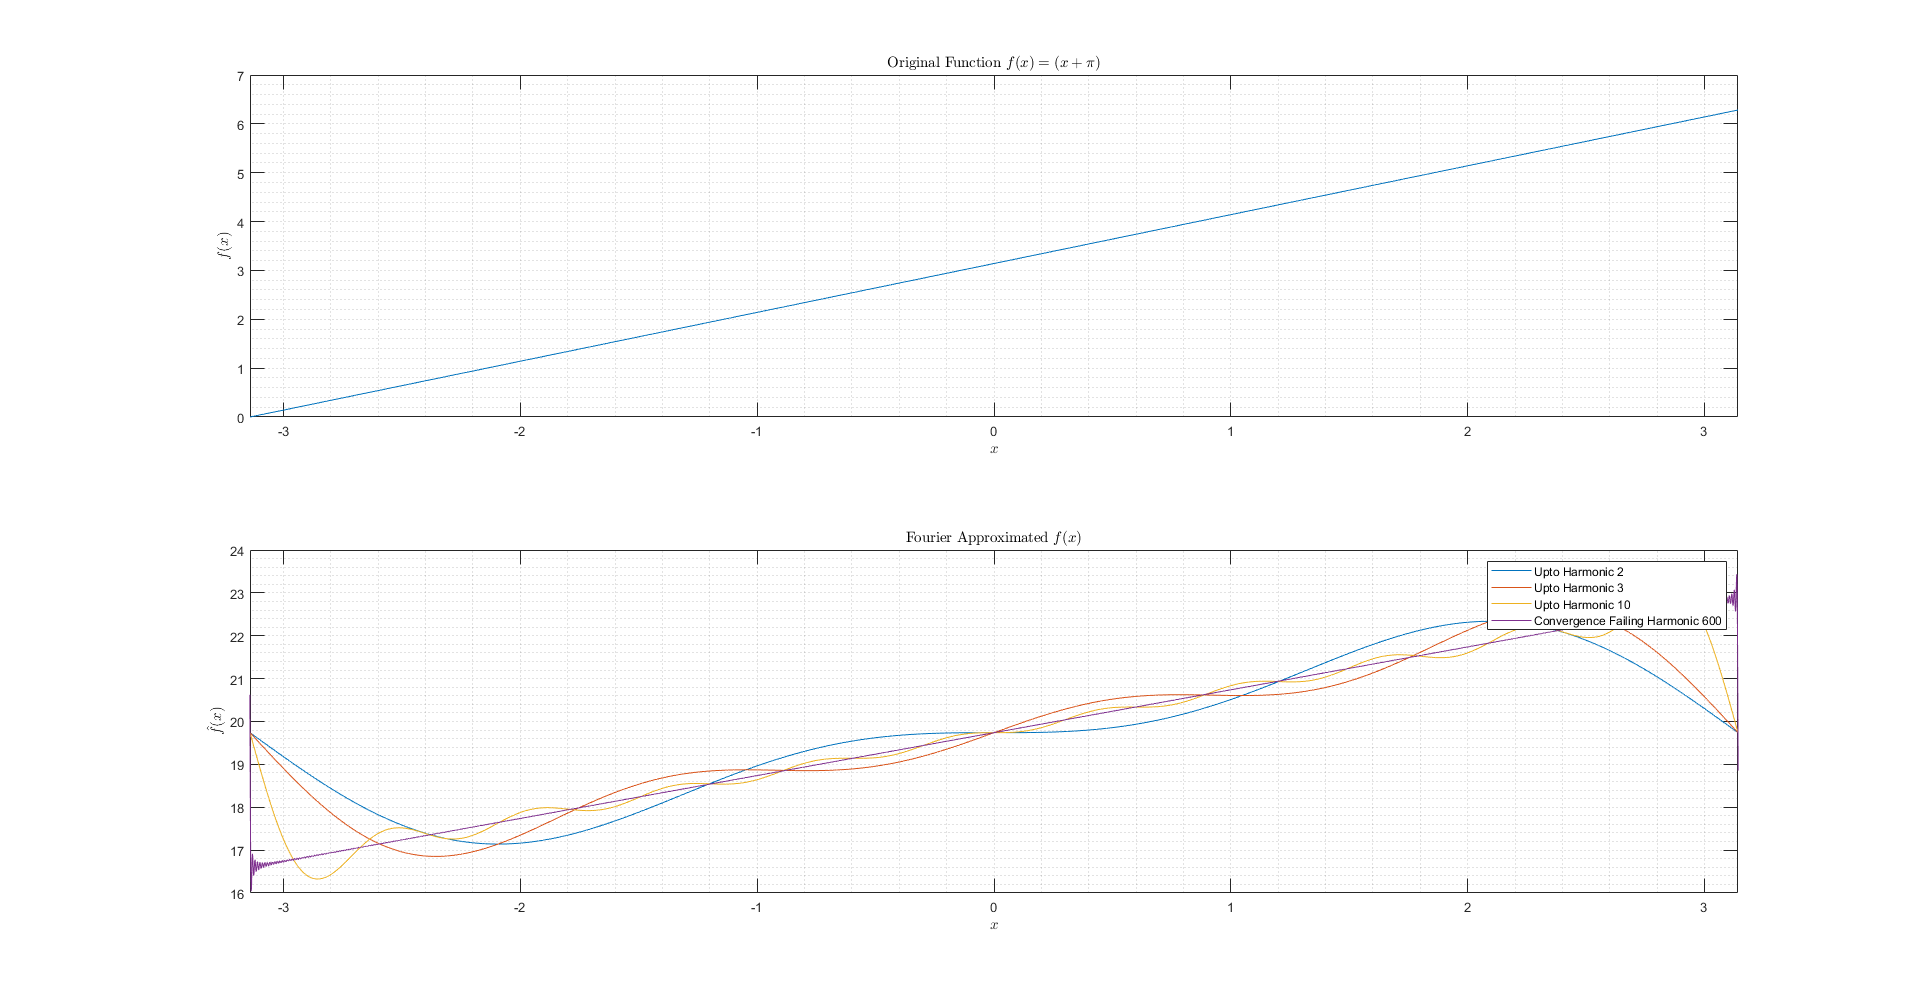
\includegraphics[scale=0.32]{Pics/Prob1.png}
    \caption{Question 1 Simulation On MATLAB}
    \label{fig:my_label}
\end{figure}
\newpage
%%%%%%%%%%%%%%%%%%%%%%%%%%%%%%%%%%%%%%%%%%%%%%%%%%%%%%%%%%%%%%%%%%%%%%%%%%%%%%%%%%%%%%%%%%%%%%%%%%%%%%%%%%%%%%%%%%%%%%%
\section*{Problem 2}
\subsection*{Given} 
\begin{flalign*}
f(x)=f(x)=\sqrt{1-\cos x}\quad \text{if}-\pi<x<\pi  &&
\end{flalign*}

\subsection*{Solution}
\begin{flalign*}
a_0=0 &&
\end{flalign*}

\begin{flalign*}
a_n=0 &&
\end{flalign*}

\begin{flalign*}
b_n=\frac{16n(-1)^n}{\pi-4\pi n^2 \sqrt2} &&
\end{flalign*}



\begin{figure}[H]

    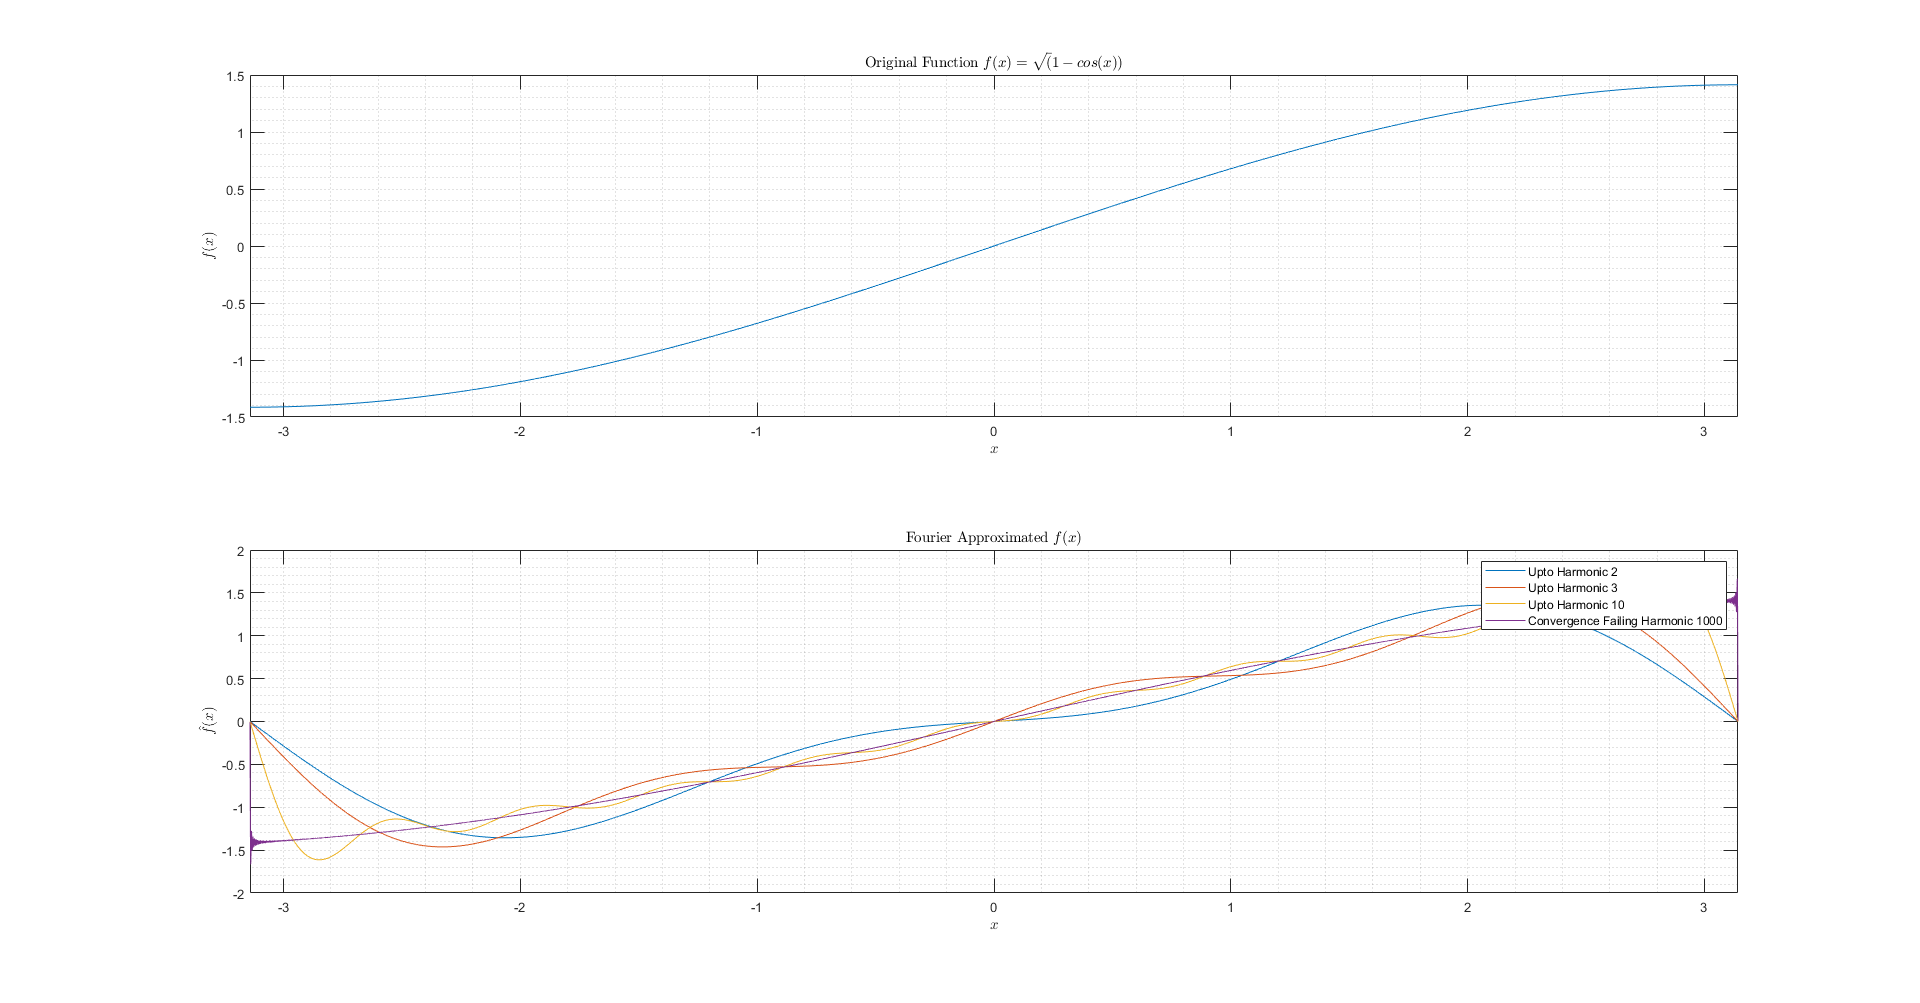
\includegraphics[scale=0.32]{Pics/Prob2.png}
    \caption{Question 2 Simulation On MATLAB}
    \label{fig:my_label}
\end{figure}
\newpage
%%%%%%%%%%%%%%%%%%%%%%%%%%%%%%%%%%%%%%%%%%%%%%%%%%%%%%%%%%%%%%%%%%%%%%%%%%%%%%%%%%%%%%%%%%%%%%%%%%%%%%%%%%%%%%%%%%%%%%%
\section*{Problem 3}
\subsection*{Given} 
\begin{flalign*}
f(x)=x\sin x \quad \text{if}-\pi<x<\pi &&
\end{flalign*}

\subsection*{Solution}
\begin{flalign*}
a_0=0 &&
\end{flalign*}

\begin{flalign*}
a_n=\frac{4n sin(n\pi)-2\pi(-1)^n (n^2-1)}{(n^2-1)^2}&&
\end{flalign*}

\begin{flalign*}
b_n=0 &&
\end{flalign*}



\begin{figure}[H]

    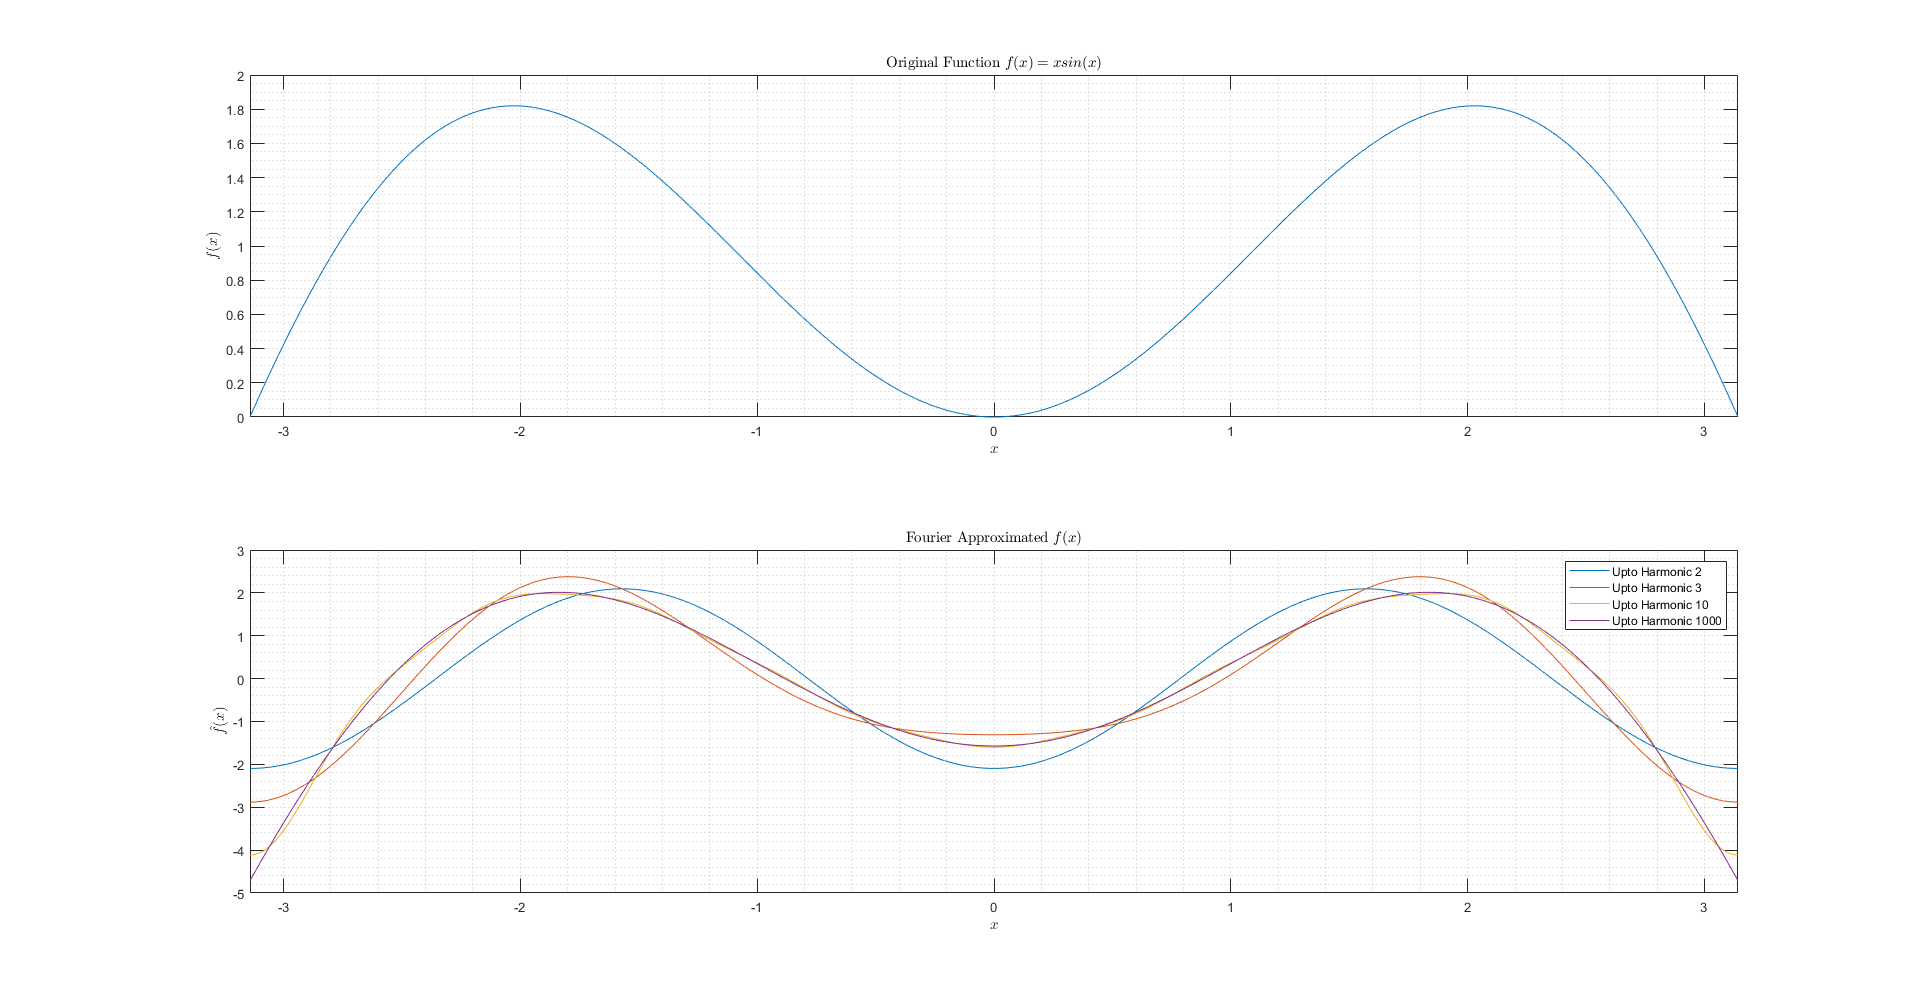
\includegraphics[scale=0.32]{Pics/Prob3.png}
    \caption{Question 3 Simulation On MATLAB}
    \label{fig:my_label}
\end{figure}
\newpage
%%%%%%%%%%%%%%%%%%%%%%%%%%%%%%%%%%%%%%%%%%%%%%%%%%%%%%%%%%%%%%%%%%%%%%%%%%%%%%%%%%%%%%%%%%%%%%%%%%%%%%%%%%%%%%%%%%%%%%%
\section*{Problem 4}
\subsection*{Given} 
\begin{flalign*}
f(x)=x\cos x \quad \text{if}-\pi<x<\pi &&
\end{flalign*}

\subsection*{Solution}
\begin{flalign*}
a_0=0 &&
\end{flalign*}

\begin{flalign*}
a_n=0 &&
\end{flalign*}

\begin{flalign*}
b_n=\frac{2\pi n(n^2-1) cos(n\pi)-2(n^2+1) sin(n\pi)}{(n^2+1)^2} &&
\end{flalign*}



\begin{figure}[H]

    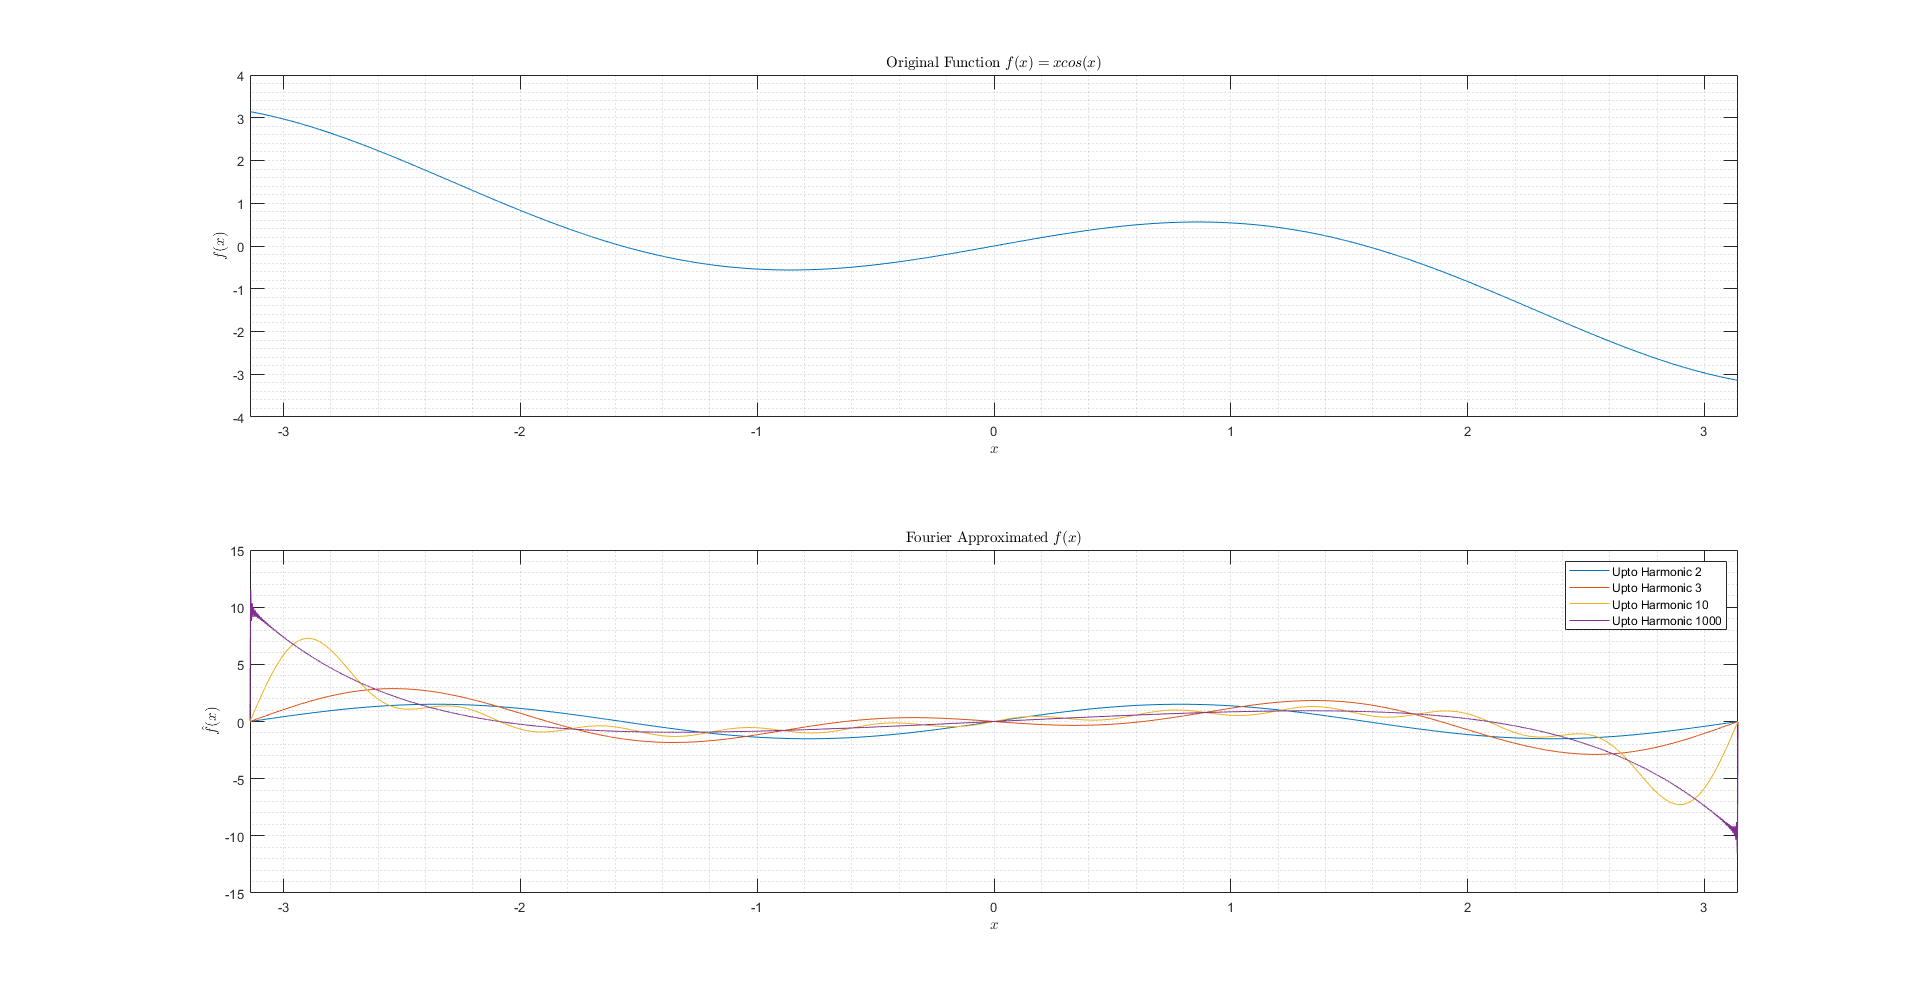
\includegraphics[scale=0.32]{Pics/Prob4.png}
    \caption{Question 4 Simulation On MATLAB}
    \label{fig:my_label}
\end{figure}
\newpage
%%%%%%%%%%%%%%%%%%%%%%%%%%%%%%%%%%%%%%%%%%%%%%%%%%%%%%%%%%%%%%%%%%%%%%%%%%%%%%%%%%%%%%%%%%%%%%%%%%%%%%%%%%%%%%%%%%%%%%%
\section*{Problem 5}
\subsection*{Given} 
\begin{flalign*}
f(x)=\mathrm{e}^{-x}\quad \text{if}\quad 0<x<2\pi \quad\text{and} \quad f(x+2\pi)=f(x) &&
\end{flalign*}

\subsection*{Solution}
\begin{flalign*}
a_0=\frac{1-e^{-2\pi}}{2\pi}&&
\end{flalign*}

\begin{flalign*}
a_n=\frac{1-e^{-2\pi}}{(n^2-1)\pi}&&
\end{flalign*}

\begin{flalign*}
b_n=\frac{n(1-e^{-2\pi})}{(n^2+1)\pi} &&
\end{flalign*}



\begin{figure}[H]

    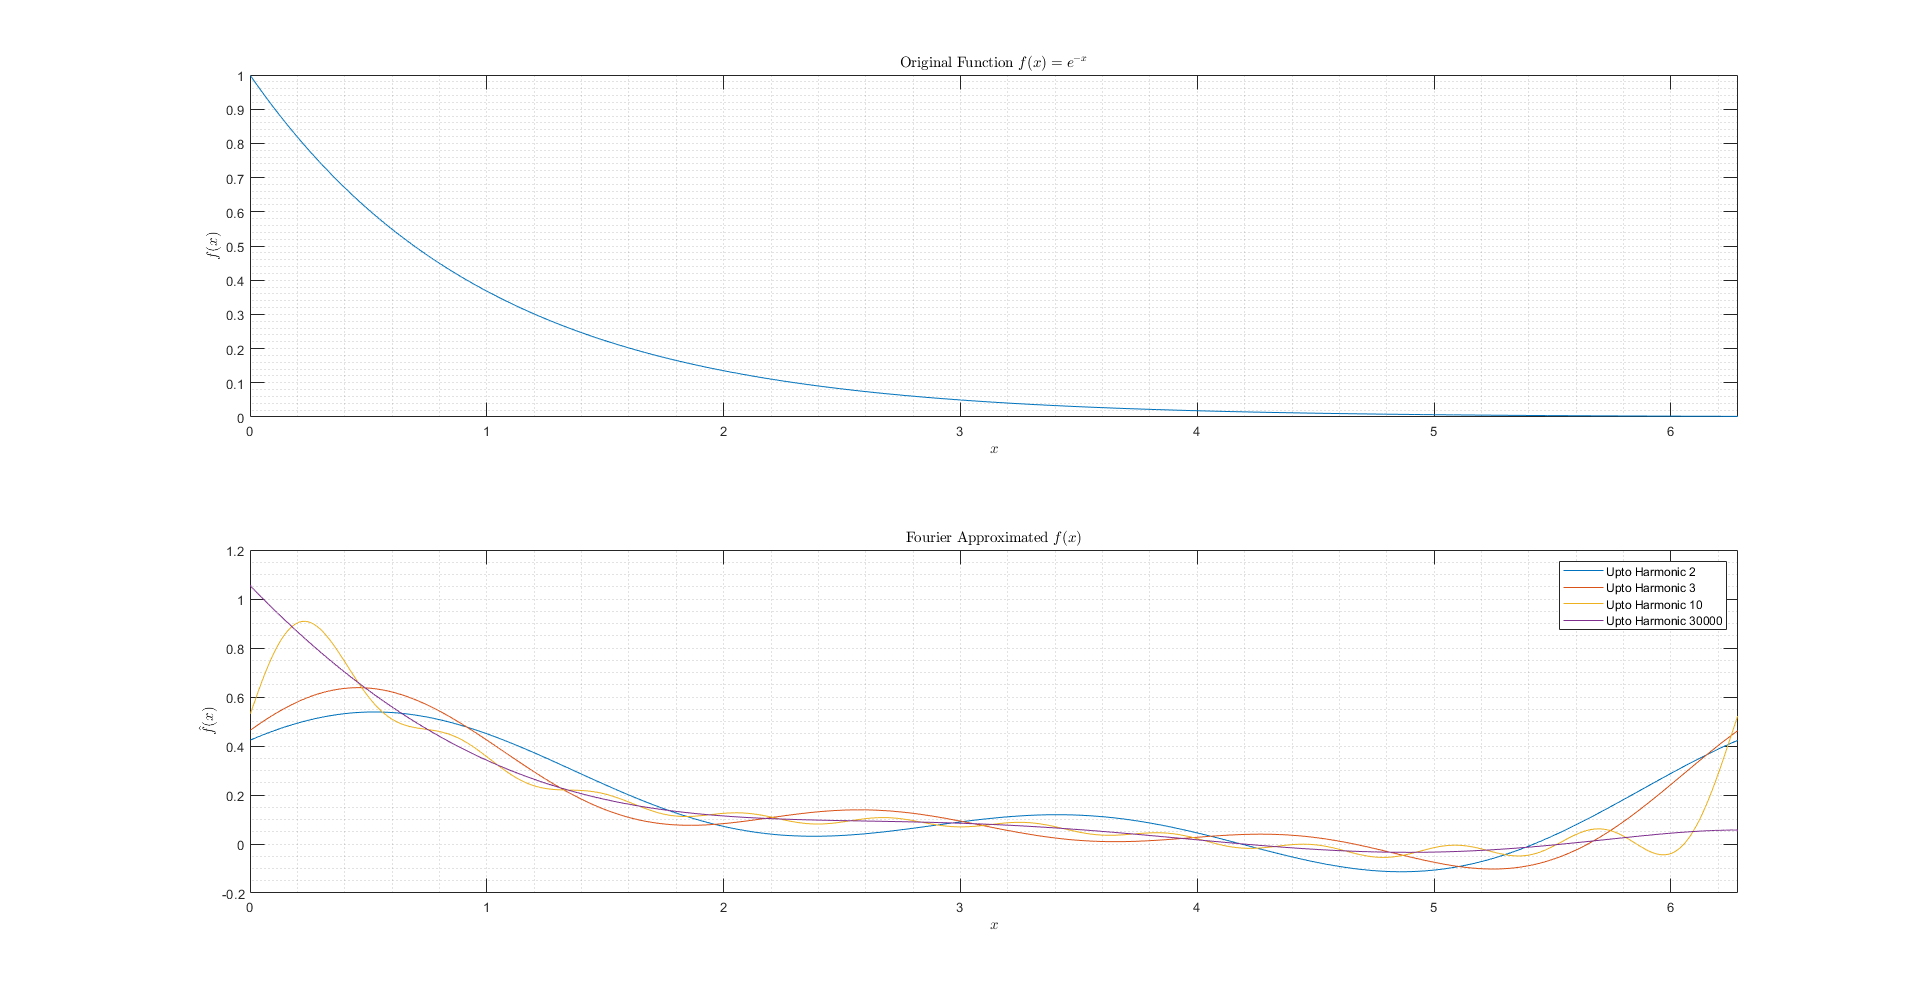
\includegraphics[scale=0.32]{Pics/Prob5.png}
    \caption{Question 5 Simulation On MATLAB}
    \label{fig:my_label}
\end{figure}
\newpage
%%%%%%%%%%%%%%%%%%%%%%%%%%%%%%%%%%%%%%%%%%%%%%%%%%%%%%%%%%%%%%%%%%%%%%%%%%%%%%%%%%%%%%%%%%%%%%%%%%%%%%%%%%%%%%%%%%%%%%%
\section*{Problem 6}
\subsection*{Given} 
A periodic function
\begin{flalign*}
f(x) = 
\begin{cases} 
\pi x &\mbox{in } 0\leq x\leq 1 \\
\pi(2-x) & \mbox{in } 1\leq x\leq 2 
\end{cases}\\
\end{flalign*}

\begin{flalign*}
a_0=\frac{\pi}{2} &&
\end{flalign*}

\begin{flalign*}
a_n=\frac{2((-1)^n-1)}{n^2\pi} &&
\end{flalign*}

\begin{flalign*}
b_n=\frac{2sin(n\pi)}{n^2\pi} &&
\end{flalign*}



\begin{figure}[H]

    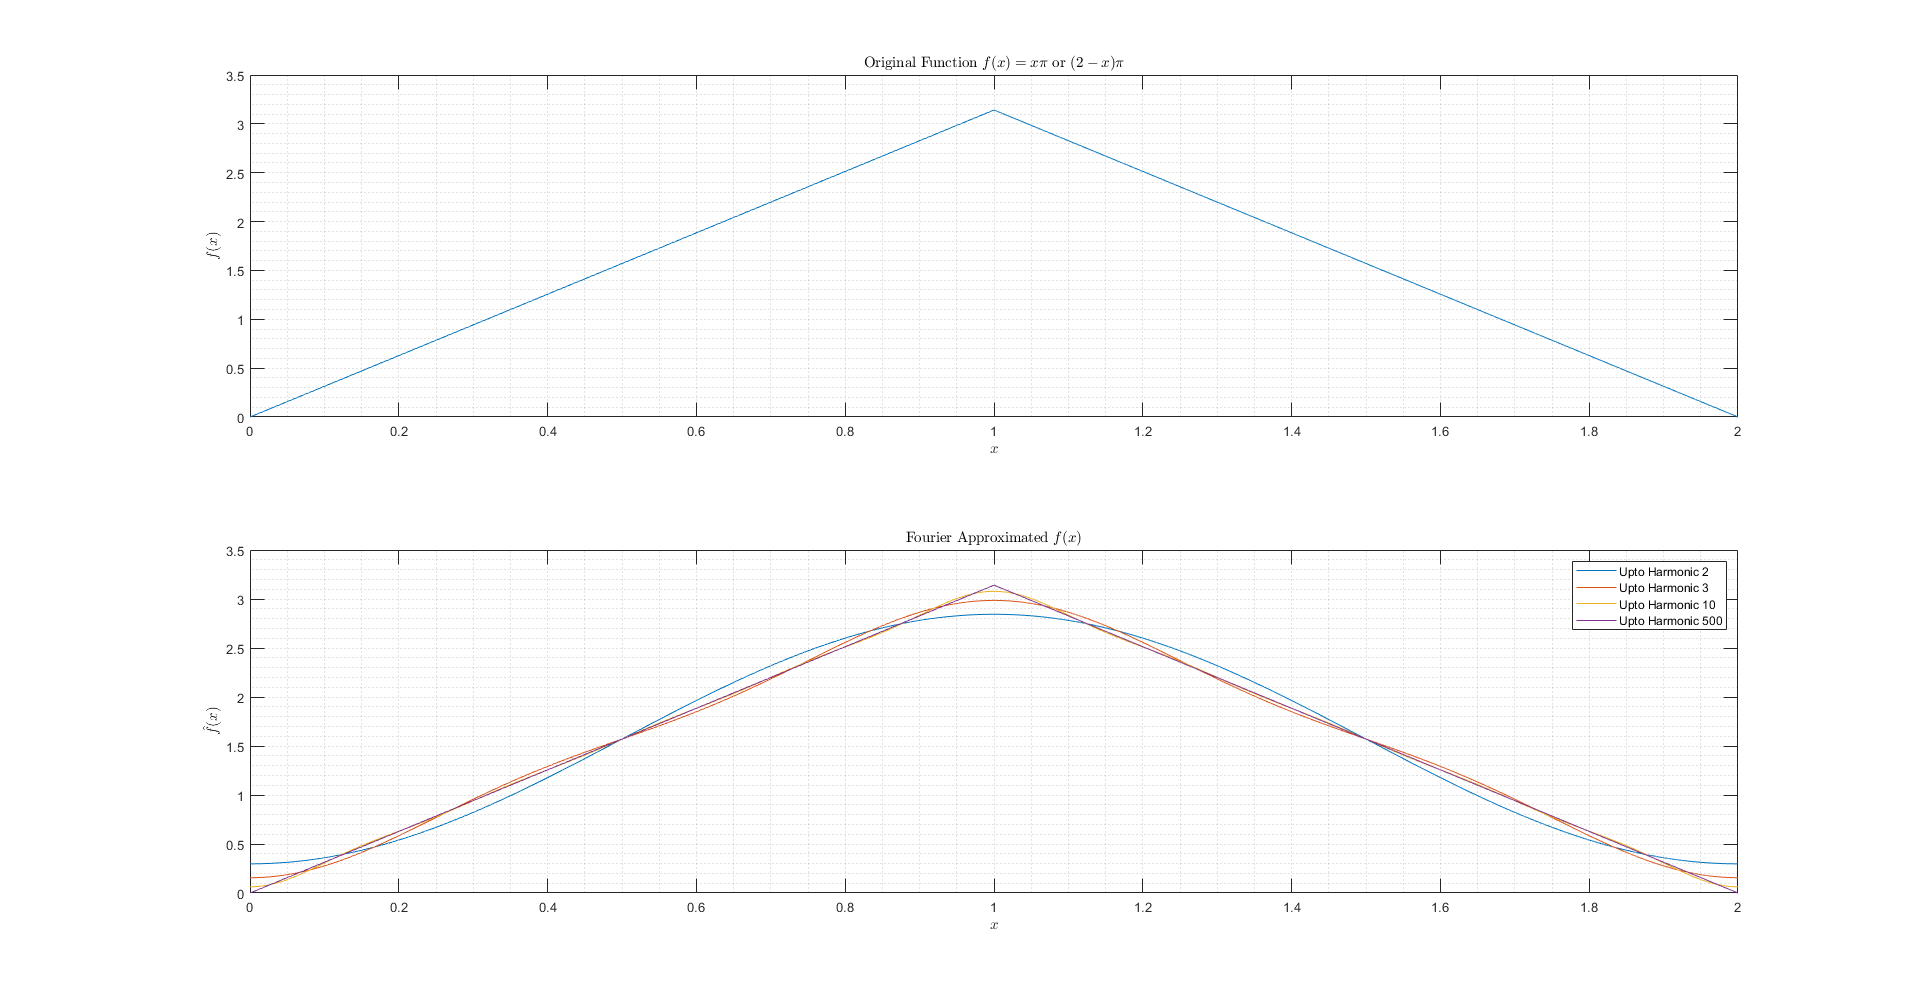
\includegraphics[scale=0.32]{Pics/Prob6.png}
    \caption{Question 6 Simulation On MATLAB}
    \label{fig:my_label}
\end{figure}
\newpage
%%%%%%%%%%%%%%%%%%%%%%%%%%%%%%%%%%%%%%%%%%%%%%%%%%%%%%%%%%%%%%%%%%%%%%%%%%%%%%%%%%%%%%%%%%%%%%%%%%%%%%%%%%%%%%%%%%%%%%%
\section*{Problem 7}
\subsection*{Given} 
When a sinusoidal voltage $V_0\sin\omega t$ is passed through a half wave 
rectifier which clips the negative portion of the wave, the resulting periodic function is 
given by


\begin{flalign*}
 v(t) = 
\begin{cases} 
\phantom{abcd} 0 &\text{for}\quad -\pi/\Omega< t< 0 \\
V_0\sin\Omega t &\text{for}\quad 0< t< \pi/\Omega
\end{cases}
\end{flalign*}\\
Develop the function.\\

\subsection*{Solution}
\begin{flalign*}
a_0=\frac{V_0}{\pi} &&
\end{flalign*}

\begin{flalign*}
a_n=\frac{((-1)^n+1)V_0}{(1-n^2)\pi} &&
\end{flalign*}

\begin{flalign*}
b_n=\frac{V_0 sin(n \pi)}{(1-n^2)\pi} &&
\end{flalign*}



\begin{figure}[H]

    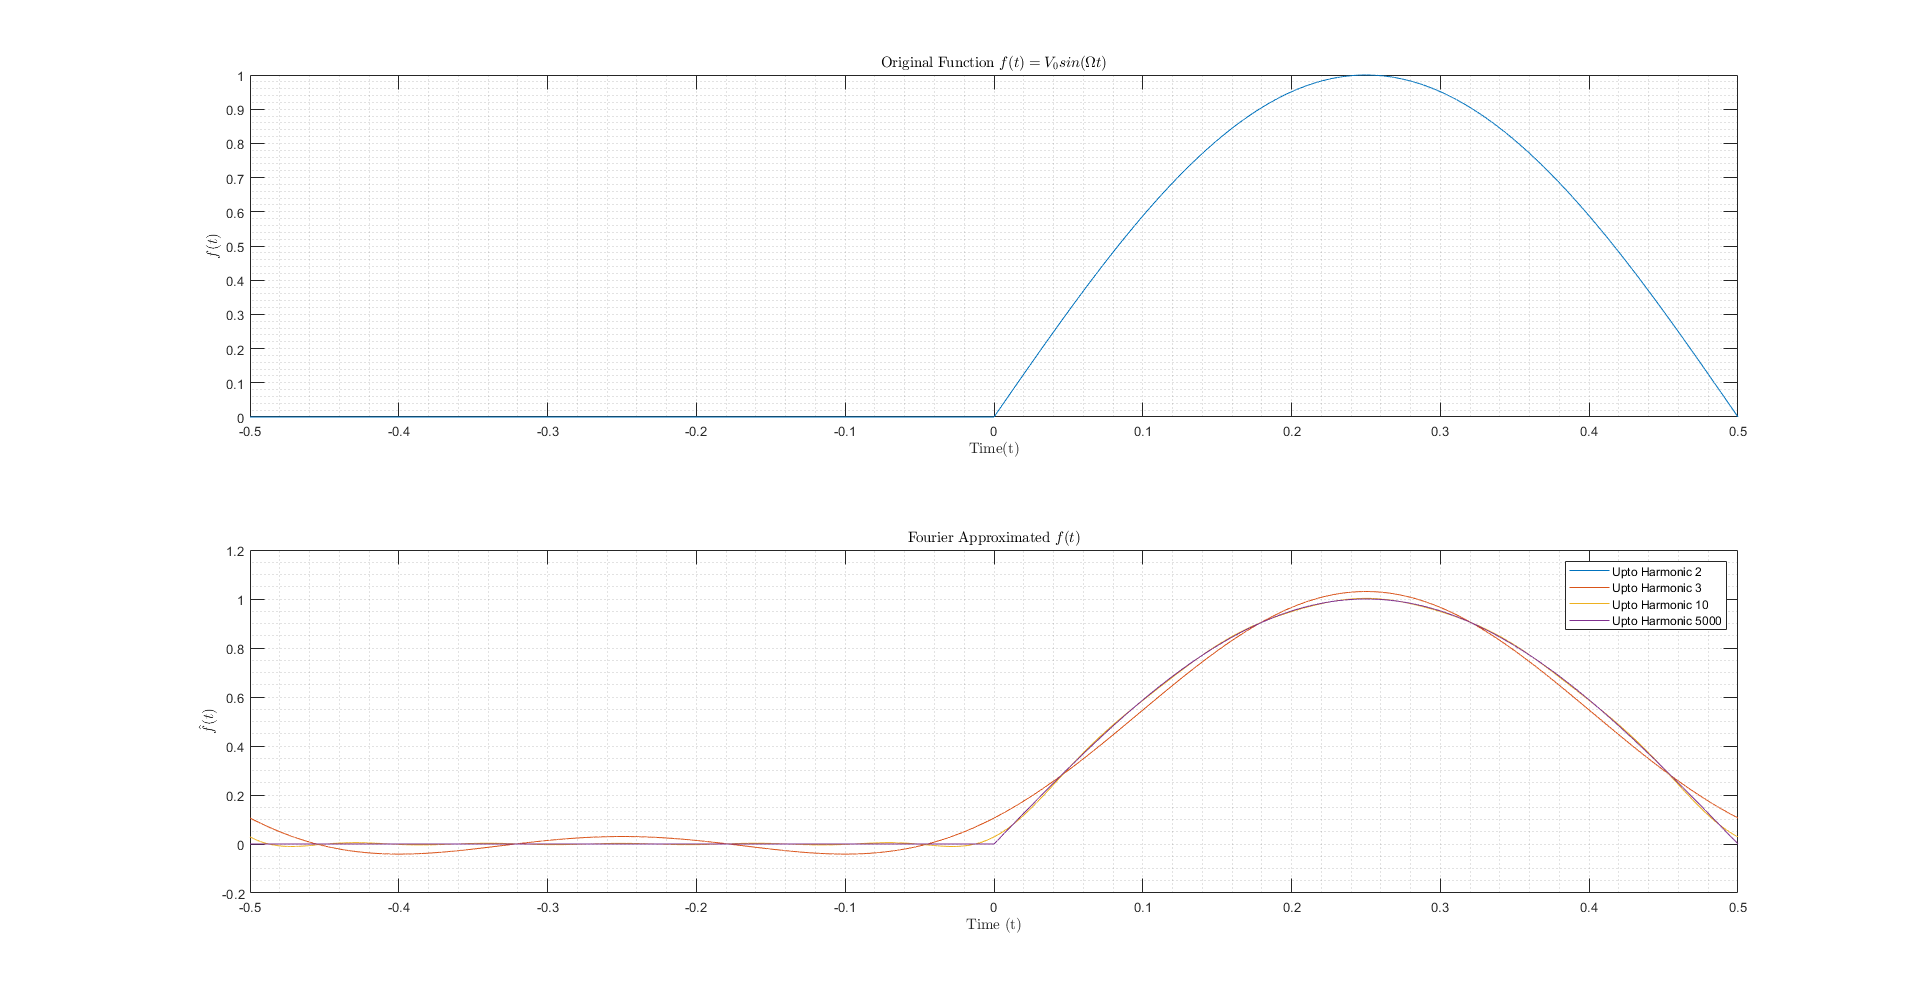
\includegraphics[scale=0.32]{Pics/Prob7.png}
    \caption{Question 7 Simulation On MATLAB}
    \label{fig:my_label}
\end{figure}

%%%%%%%%%%%%%%%%%%%%%%%%%%%%%%%%%%%%%%%%%%%%%%%%%%%%%%%%%%%%%%%%%%%%%%%%%%%%%%%%%%%%%%%%%%%%%%%%%%%%%%%%%%%%%%%%%%%%%%%

\end{document} 
